%----------------------------------------
% Write your notes here
%----------------------------------------

\section{Naive Bayes}
\subsection{Basic Ideas}
Say we want to predict a class $c$ given features $x$. For example, say we want to classify emails as spam or not spam. Our classes $c$ would be $\{0,1\}$ where 0 represents not spam and 1 represents spam. Our features $x$ would consist of values $\in \{0,1\}$ representing whether a word is present or not.

What we want to predict is $p(c|x)$ or the probability of a class $c$ given the features $x$.

Using Bayes' Rule we can get:
\begin{equation}
	p(c|x) = \frac{p(x|c)p(c)}{p(x)}
\end{equation}
Here, $p(x|c)$ represents the probability of seeing all words given the class $c$.

We also make the "naive" assumption of independence and assume that each word occurrence $p(x_i|c)$ is a "coin flip" with a Bernoulli distribution. Thus we get:
\begin{equation}
	p(c|x) = \frac{\prod p(x_i|c) p(c)}{p(x)}
\end{equation}
\begin{equation}
    p(x_j|c) = \theta_{jc}^{x_j} (1 - \theta_{jc})^{1-x_j}
\end{equation}

Here, $\theta$ is just shorthand for probabilities s.t. $\theta_{jc}$ is the probability of the $j$th word in class $c$.

If we take logs then we get:
\begin{equation}
\log p(c|x) = \sum_{j} \log [\theta_{jc}^{x_j} (1-\theta_{jc})^{1-x_j}] + \log \frac{\theta_c}{p(x)}
\end{equation}
\begin{equation}\label{eq:5}
\log p(c|x) = \sum_{j} x_j \log \frac{\theta_{jc}}{1 - \theta_{jc}} + \sum_j \log (1 - \theta_{jc}) + \log \frac{\theta_c}{p(x)}
\end{equation}

Where, using the product rule, we can get:
\begin{equation}
p(x) = \sum_c p(x,c) = \sum_c p(x|c) p(c)
\end{equation}

Looking quickly at the computational cost for this equation, we know that the first term is dependent on the number of words present in the document we're looking at, and the second term is dependent on the size of the vocabulary.

If there are two classes, with the possible values of $c$ being 1 or 0, then we can represent the Naive Bayes classifier in log odds form as follows:
\begin{equation}
\log\frac{p(c=1|x)}{p(c=0|x)}
\end{equation}
If the log odds is greater than 0, then we predict $c = 1$, and if it's less than 0, we predict $c = 0$.

Using our equation (\ref{eq:5}) we get:
\begin{equation}
\log\frac{p(c=1|x)}{p(c=0|x)} = \sum_j x_j \log\frac{\theta_{j1}(1-\theta_{j0})}{\theta_{j0}(1-\theta_{j1})} + \sum_j \log\frac{1-\theta_{j1}}{1-\theta_{j0}} + \log{\theta_1}{\theta_0}
\end{equation}

We can assign the following values to simplify our classifier:
\begin{equation}
w_j = \log\frac{\theta_{j1}(1-\theta_{j0})}{\theta_{j0}(1-\theta_{j1})}
\end{equation}
\begin{equation}
w_0 = \sum_j \log\frac{1-\theta_{j1}}{1-\theta_{j0}} + \log{\theta_1}{\theta_0}
\end{equation}
\begin{equation}
\log\frac{p(c=1|x)}{p(c=0|x)} = \mathbf{w} \cdot \mathbf{x} + w_0
\end{equation}

If we precompute $w_0$ then the computational cost is just the number of nonzero words.

\subsection{Finding \texorpdfstring{$\theta_j$}{Thetas}}
To explain how to find individual $\theta$ values for our classifier, we did a derivation of the probability of seeing $n$ heads for $N$ coin flips, since a similar concept is applied to the probabilities of seeing words in documents, or other applications of the classifier.

We have the the probability of seeing $n$ heads given $\theta$ is:
\begin{equation}
p(n|\theta) = C \theta^n (1-\theta)^{N-n}
\end{equation}

We can take the log for likelihood, then take the derivative and set to zero to find the max likelihood.
\begin{equation}
\mathcal{L} = \log p(n|\theta) = \log C + n \log {\theta} + (N - n) \log (1 - \theta)
\end{equation}
\begin{equation}
0 = \frac{\partial \mathcal{L}}{\partial \theta} = \frac{n}{\theta} + \frac{N-n}{1-\theta}
\end{equation}
\begin{equation}
\frac{n}{\theta} = \frac{N-n}{1-\theta}
\end{equation}
\begin{equation}
n - n\theta = N\theta - n\theta
\end{equation}
\begin{equation}
\theta = \frac{n}{N}
\end{equation}

Using this, then we can get:
\begin{equation}
\theta_{j1} = \frac{n_{j1}}{n_1} = \frac{\textnormal{\# of spam docs w/ word j}}{\textnormal{total \# of spam docs}}
\end{equation}
\begin{equation}
\theta_{1} = \frac{n_{1}}{N} = \frac{\textnormal{\# of spam docs}}{\textnormal{total \# docs}}
\end{equation}

\subsection{Time and Space}
With $N$ documents, $c$ classes, and $k$ different words, the training time for a Naive Bayes classifier is $O(N\cdot \overline{k})$ where $\overline{k}$ is the average number of words in a document. The required space \textit{seems} like it would be $O(k \cdot c)$ but storing using a sparse data structure would save space.

\section{Logistic Regression}
\subsection{The Logistic Function}
Say we start with a predictor that has the same form as the Naive Bayes classifier that we ended with:
\begin{equation}
\log \frac{p}{1-p} = \textbf{w} \cdot \textbf{x}
\end{equation}

(Note: There is an implicit intercept in this equation that we are ignoring.)

Using this predictor, we can get some useful values for $p(x|w)$ and $1-p(x|w)$:

\begin{equation}\label{eq:20}
\frac{p}{1-p} = e^{\textbf{w} \cdot \textbf{x}}
\end{equation}
\begin{equation}
p = e^{w \cdot x} - pe^{w \cdot x}
\end{equation}
\begin{equation}
p(1+e^{w \cdot x}) = e^{w \cdot x}
\end{equation}
\begin{equation}\label{eq:24}
p = \frac{e^{w \cdot x}}{1+e^{w \cdot x}}
\end{equation}
\begin{equation}\label{eq:25}
p(x|w) = \frac{1}{1+e^{-w \cdot x}}
\end{equation}
\begin{equation}\label{eq:26}
1-p(x|w) = 1 - \frac{1}{1+e^{-w \cdot x}} = \frac{1}{1+e^{w \cdot x}}
\end{equation}

Equation \ref{eq:25} is a sigmoid function that when plotted gives us the S-shaped logistic curve, as seen below:
\begin{figure}[ht]
  \begin{center}
    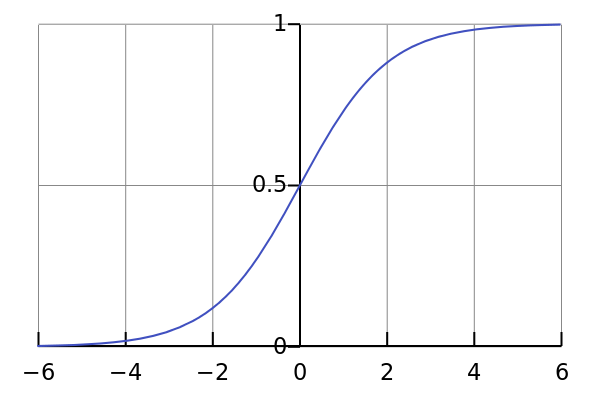
\includegraphics[width=0.5\textwidth]{figures/Logistic-curve.png}
    \caption{https://en.wikipedia.org/wiki/Sigmoid\_function}
    \label{fig:logistic}
  \end{center}
\end{figure}

\subsection{Determining the Model}
Say we have a set of labels $y_i \in {0,1}$ where 1 represents spam and 0 represents ham, and a set of documents $x_i$.

Then we get likelihood as follows, where $p_i = p(x_i|w)$:
\begin{equation}
p(D|w) = \prod_i p_i^{y_i} (1-p_i)^{1-y_i}
\end{equation}

Taking the log likelihood, we get:
\begin{equation}
\mathcal{L} = -\log p(D|w)
\end{equation}
\begin{equation}
\mathcal{L} = -\sum_i \{y_i \log p_i + (1-y_i)\log (1-p_i)\}
\end{equation}
\begin{equation}
\mathcal{L} = -\sum_i \{y_i \log \frac{p_i}{1-p_i} + \log (1-p_i)\}
\end{equation}

From \ref{eq:20} and \ref{eq:26} above, we can get:

\begin{equation}
\mathcal{L} = -\sum_i \{y_i w \cdot x - \log(1+e^{w \cdot x}) \}
\end{equation}

Then finding maximum likelihood:

\begin{equation}
0 = \frac{\partial\mathcal{L}}{\partial w_k} = -\sum_i \{y_i x_{ik} - \frac{1}{1+e^{w \cdot x_i}} e^{w \cdot x_i} x_{ik} \}
\end{equation}

Using equation \ref{eq:24} we get:

\begin{equation}
0 = -\sum_i \{ y_i - p_i \} x_{ik}
\end{equation}
\begin{equation}
0 = -\sum_i \{ y_i - \frac{1}{1 + e^{-w \cdot x}} \} x_{ik}
\end{equation}

There is no closed form solution to this equation, so we use gradient descent:

\begin{equation}
w \leftarrow w - \eta \frac{\partial\mathcal{L}}{\partial w}
\end{equation}

In matrix form we get:

\begin{equation}
w \leftarrow w + \eta X^T (y - p)
\end{equation}

Which can also be represented in component form as:
\begin{equation}
w_{k} \leftarrow w_{k} + \eta \sum_i (y_i - p_i) x_{ik}
\end{equation}


\subsection{Side Note: Regularized Logistic Regression}
If we don't want the weights in our logistic regression model to get too big, we can use regularization. Then our likelihood equation becomes:

\begin{equation}\label{eq:38}
\mathcal{L} = -\sum_i \{ y_i \log p_i + (1-y_i) \log (1-p_i) \} + \frac{1}{2} \lambda ||w||^2
\end{equation}
\begin{equation}\label{eq:39}
\frac{\partial\mathcal{L}}{\partial w} = -\sum_i (y_i - p_i) x_{ik} + \lambda w_k
\end{equation}

The last term in (\ref{eq:38}) is our regularization term.

Then our update rule becomes:
\begin{equation}
w_k \leftarrow w_k - \eta \frac{\partial\mathcal{L}}{w_k} = w_k + \eta \sum_i (y_i - p_i) x_{ik} - \lambda w_k
\end{equation}
\begin{equation}
w_k \leftarrow (1-\eta\lambda)w_k + \eta \sum_i (y_i - p_i) x_{ik}
\end{equation}

Essentially what we're doing in the update is shrinking the weights first before moving against the gradient the updating our weights.

\section{Evaluating Classifiers}
There are a couple of different metrics and terms that are often used to evaluate classifiers:

\begin{itemize}
\item \textbf{accuracy}: The fraction of times you predict the correct label.
\item \textbf{calibration}: Measures how often an event with predicted probability $p$ occurs. 

\item \textbf{confusion matrix}: a way of representing predicted and actual values.
\begin{center}
\begin{tabular}{ |c|c|c| } 
 \hline
  & \multicolumn{2}{|c|}{predicted} \\
  \hline
  actual & 1 & 0 \\
  \hline
  1 & true positive (TP) & false negative (FN) \\
  \hline 
  0 & false positive (FP) & true negative (TN) \\
 \hline
\end{tabular}
\end{center}

\item \textbf{precision}: The fraction of positive predictions that are true. Can also be represented as $\frac{\textnormal{TP}}{\textnormal{TP}+\textnormal{FP}}$
\item \textbf{recall} (aka true positive rate): fraction of true examples that we predict to be positive. $\frac{\textnormal{TP}}{\textnormal{TP}+\textnormal{FN}}$
\item \textbf{false positive rate}: fraction of false examples that are predicted positive. $\frac{\textnormal{TP}}{\textnormal{TP}+\textnormal{FN}}$

\item \textbf{receiver operator characteristic curve (ROC)}: we can plot the TPR (probability of true detection) vs. FPR (probability of a false alarm) and by changing our probability threshold, we can get a curve, as shown below:
\begin{figure}[ht]
  \begin{center}
    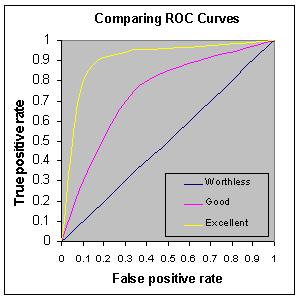
\includegraphics[width=0.5\textwidth]{figures/roc-curve.jpg}
    \caption{
      http://gim.unmc.edu/dxtests/roc3.htm}
    \label{fig:roc}
  \end{center}
\end{figure}

\item \textbf{area under curve (AUC)}: the area under the ROC curve is equivalent to the accuracy for a balanced classification

\end{itemize}

\section{"Guest Lecture": Computational Social Science: Exciting Progress and Future Challenges}
\subsection*{Speaker: Duncan Watts}

\subsection{Introduction}
A problem of particular interest in social science is the \textbf{"micro-macro" or emergence problem}. This is the phenomena of collective social behavior that spawns from an individual level. Unfortunately, it's hard to study this problem empirically, especially on a "macro" scale. However, the advent of the Internet means that there is a dramatic increase in the scale, scope, and granularity of data available. Web platforms also allow for an increase in the speed and scale of experiments.

In this talk, we looked at computational social science from two main examples: "big data" social contagion and "small data" virtual lab experiments. 

\subsection{Social Contagion using Big Data}
In this section of the talk, we look at how things go viral. When we talk about "viral" or "social contagion," our concept of this term comes from biological/epidemiological ideas of a multigenerational branching spread. But historically, S-shaped curves have always been used to represent social data and infer "diffusion" events and virality.

There are two main problems with this historical approach:
\begin{enumerate}
\item An S-shaped curve can result from many different processes (e.g. marketing efforts, population heterogeneity)
\item We usually only see and collect data for successful diffusion events, so we have few examples of unsuccessful ones.
\end{enumerate}

Exploring social contagion requires the use of individual-level data and data from unsuccessful attempts. The web helps solve some of these problems. The following are some examples of projects that involve the web, big data, and social contagion.

\subsubsection{Online Diffusion Project (2012: Goel, Watts, Goldstein)}
Associated Paper: S. Goel, D. J. Watts, and D. G. Goldstein, \href{http://dl.acm.org/citation.cfm?id=2229058}{The structure of online diffusion networks}. In Proceedings of the 13th ACM Conference on Electronic Commerce (EC '12). 2012.

\bigskip
This project involved 6 unrelated projects that were all designed in an attempt to go viral. There were consistent diffusion patterns across all the projects. They found that 99\% of adoptions are $\leq$ 1 "hop" from the seed, or origin/source, suggesting that there isn't much virality in spreading.

\subsubsection{"Structural Virality" Project (2015: Goel, Anderson, Hofman, Watts)}
Associated Paper: S. Goel, A. Anderson, J. Hofman, and D. J. Watts,  \href{http://pubsonline.informs.org/doi/pdf/10.1287/mnsc.2015.2158}{The Structural Virality of Online Diffusion}. Management
Science 62(1):180-196. 2015.

\bigskip
This project looked at every video, news story, image, and petition on Twitter over a timespan of 12 months. This was about 1.4 billion different "events". They restricted this dataset to only "popular" things by taking only events that had over 100 retweets, resulting in about 350,000 items to look at.

They looked at the average shortest path length for nodes in the viral structure to classify the structure. Structures with an average shortest path length of 2 were "broadcast" and those with an average shortest path length of log(n) were "viral".

What they found was that there are all sorts of patterns and structures in the "virality" of a viral event's spread that is unrelated to time scale. They found that popularity $\neq$ virality. Popularity is usually driven by celebrities, or the individuals that are the largest source of broadcasting.

\subsubsection{How Predictable are Cascades? (2016: Martin, Hofman, Sharma, Anderson, Watts)}
Associated Paper: T. Martin, J. Hofman, A. Sharma, A. Anderson, and D. J. Watts, \href{http://www2016.net/proceedings/proceedings/p683.pdf}{Exploring Limits to Prediction in Complex Social Systems}.  Proceedings of the 25th ACM International World Wide Web Conference (WWW). 2016.

\bigskip
This paper looked at whether popularity/cascade size is predictable. What they found was that using only past success as a predictor could get the same result as a more complex model with more features. This suggests that there's an asymptotical limit to how well and how much popularity/cascade size can be predicted, and that perhaps sociological theories are not enough to predict behavior in these cases because there is too much randomness.

\subsection{Virtual Labs}
Traditional physical behavioral lab experiments have a lot of limitations (validity in external environments, expensive, slow.) Virtual labs allow for more realism, scale, and duration in the experimental design space.

We went over 3 examples of how virtual labs allow for expansion in scale, realism, and time.

\subsubsection{Scale: Music Lab (2006: Salganik, Dodds, Watts)}
Associated Paper: M. J. Salganik, P. S. Dodds, and D. J. Watts, \href{https://www.princeton.edu/~mjs3/salganik_dodds_watts06_full.pdf}{"Experimental study of inequality and unpredictability in an artificial cultural market."} Science, 311:854-856, 2006.

\bigskip
The \href{http://www.princeton.edu/~mjs3/musiclab.shtml}{Music Lab} was an experiment that looked at social influence and market dynamics, and involved getting thousands of volunteers recruited from social media to participate in a web app that was designed expressly for the purposes of the experiment. This experiment is an example of how virtual labs allow for massive increases in the scale of an experiment.

\subsubsection{Realism: Crisis Mapping in the Lab (2016: Mao, Mason, Suri, Watts)}
Associated Paper: A. Mao, W. Mason, S. Suri, and D. J. Watts, \href{http://journals.plos.org/plosone/article?id=10.1371/journal.pone.0153048}{An Experimental Study of Team Size and Performance on a Complex Task}.  PLoS ONE 11(4). 2016.

\subsubsection{Time: Month-long Prisoner's Dilemma Experiment}
Associated Paper: A. Mao, L. Dworkin, S. Suri, D. J. Watts, \href{http://www.nature.com/articles/ncomms13800}{Resilient cooperators stabilize long-run cooperation in the finitely repeated Prisoner’s Dilemma}. 2017.